\documentclass[14pt, a4paper]{extarticle}	
\usepackage{GOST}

\makeatletter
\renewcommand\@biblabel[1]{#1.}
\makeatother


\graphicspath{{images/}}

\begin{document}
\begin{table}[ht]
	\centering
	\begin{tabular}{|c|p{400pt}|} 
	\hline
		\begin{tabular}[c]{@{}c@{}} 
\includegraphics[scale=0.85]{b_logo	} \\\end{tabular} &
		\footnotesize\begin{tabular}[c]{@{}c@{}}\textbf{Министерство~науки~и~высшего~образования~Российской~Федерации}\\\textbf{Федеральное~государственное~бюджетное~образовательное~учреждение}\\\textbf{~высшего~образования}\\\textbf{«Московский~государственный~технический~университет}\\\textbf{имени~Н.Э.~Баумана}\\\textbf{(национальный~исследовательский~университет)»}\\\textbf{(МГТУ~им.~Н.Э.~Баумана)}\\\end{tabular}  \\
	\hline
	\end{tabular}
\end{table}
\noindent\rule{\textwidth}{4pt}
\noindent\rule[14pt]{\textwidth}{1pt}
\hfill 
\noindent
\makebox{ФАКУЛЬТЕТ~}%
\makebox[\textwidth][l]{\underline{~~~~~«Информатика и системы управления»~~~~~~~~~~~~~~~~~~~~~~~~~~~~}}%
\\
\noindent
\makebox{КАФЕДРА~}%
\makebox[\textwidth][l]{\underline{~«Программное обеспечение ЭВМ и информационные технологии»}}%

\begin{center}
	\vspace{1.5cm}
	{\bf\huge Расчетно-пояснительная записка\par}
	{\bf\Large к курсовой работе\par}
	\vspace{0cm}
\end{center}


\noindent
\makebox{\large{\bf Тема:}~~~}
\makebox[\textwidth][l]{\large\underline{~Реализация драйвера виртуального сетевого интерфейса}}\\

\noindent
\makebox{\large{\bf Дисциплина:}~~~}
\makebox[\textwidth][l]{\large\underline{~Операционные системы}}\\

\vspace{1cm}
\noindent
\begin{tabular}{l c c c c c}
    Студент      & ~ИУ7-75Б~       & \hspace{2.5cm} & \hspace{3.5cm}                 & &  П.К. Хетагуров \\\cline{2-2}\cline{4-4} \cline{6-6} 
    \hspace{3cm} & {\footnotesize(Группа)} &                & {\footnotesize(Подпись, дата)} & & {\footnotesize(И.О. Фамилия)}
\end{tabular}

\vspace{0.5cm}

\noindent
\begin{tabular}{l c c c c}
    Руководитель проекта & \hspace{3.3cm}   & \hspace{3.5cm}              & & Н.Ю. Рязанова \\\cline{3-3} \cline{5-5} 
    \hspace{3cm}  &                & {\footnotesize(Подпись, дата)} & & {\footnotesize(И.О. Фамилия)}
\end{tabular}

\begin{center}	
	\vfill
	\large \textit {Москва, 2021}
\end{center}

\thispagestyle {empty}
\pagebreak

\setcounter{page}{3}

% СОДЕРЖАНИЕ 
\clearpage
\tableofcontents

\clearpage
\section*{Введение}
\addcontentsline{toc}{section}{Введение}


	Современные вычислительные системы сложно представить без поддержки интернет-сетей. На одном устройстве может быть доступ к различным подсетям по различным сетевым интерфесам и каналам передачи данных. Доступ к различным сетевым интерфейсам возможен на уровне пользователя, однако это требует от пользовательского ПО введения дополнительных критериев выбора сетевых интерфейсов. В данной работе рассматриваются вопросы разработки собственного виртуального интерфейса, который позволял бы пользователю абстрагироваться от выбора конкретного сетевого интерфейса. Совмещение нескольких сетевых интерфейсов в один облегчает доступ к нескольким подсетям со стороны некоторых прикладных приложений.\\
\indent Так как сетевой интерфейс может быть определен в системе только с помощью загружаемого модуля ядра, то данная работа будет основана на анализе и разработке такого загружаемого модуля.


\clearpage
\section{Аналитический раздел}
\subsection{Постановка задачи}
В соответствии с заданием на курсовую работу необходимо разработать
и реализовать драйвер виртуального сетевого интерфейса, реализующий создание виртуального сетевого интерфейса для распределения пакетов по уже существующим сетевым интерфейсам. \\
\indent Для достижения цели курсовой работы необходимо решить следующие задачи:
\begin{itemize}
	\item проанализировать работу сетевой подсистемы Linux;
	\item проанализировать функции и структуры ядра, позволяющие реализовать сетевой интерфейс;
	\item разработать необходимые модули;
	\item реализовать загружаемый модуль ядра;
	\item протестировать реализованное ПО.
\end{itemize}
\indent \indent Разрабатываемое ПО должно перенаправлять пакеты, пришедшие на виртуальный интерфейс по указанным интерфейсам в зависимости от IP назначения пакета.


\subsection{Сетевые интерфейсы и устройства}
Для доступа к сетевым устройствам используются так называемые сетевые интерфейсы. Они являются основой сетевой подсистемы Linux. Все сетевое взаимодействие в Linux происходит через сетевые интерфейсы. Любые данные, которые компьютер отправляет в сеть или получает из сети проходят через сетевой интерфейс. \\
\indent Сетевые устройства выделяют сетевые устройства как специфический тип \cite{ldd-trans}\cite{ldd-orig}. На практике сетевые устройства являются символьными. \\
\indent Однако интерфейсы это не файлы устройств и их нет в каталоге /dev. Интерфейсы создаются динамически и не всегда связаны с сетевыми картами. Например интерфейс ppp0 - это интерфейс VPNа, организованного по протоколу PPTP, а интерфейс lo это виртуальная сетевая карта с адресом localhost (127.0.0.1). Такие интерфейсы называются виртуальными. \\
\indent Таким образом сетевые интерфейсы скрывают детали реализации конкретного сетевого устройства, прикладное программное обеспечение, обращаясь к сетевому интерфейсу не учитывает детали реализации конкретных сетевых устройств. Однако в Linux существует общепринятая схема именования сетевых интерфейсов, состоящая из префикса типа сетевого устройства и заканчивающаяся номером иакого устройства. Примеры наименования интерфейсов:
\begin{itemize}
	\item eth0 --- первый сетевой интерфейс к карте Ethernet или картам WaveLan (Radio Ethernet);
	\item wlan0 --- сетевой интерфейс wi-fi адаптера;
	\item  lo --- сетевой интерфейс к виртуальной сетевой карте с адресом localhost (127.0.0.1);
	\item  enp1s3 --- четвертый сетевой  интерфейс второй группы к карте Ethernet или картам WaveLan (Radio Ethernet).
\end{itemize}
Интерфейсы создаются автоматически для каждого обнаруженного сетевого устройства при загрузке ядра ОС. \\
\indent Каждый интерфейс характеризуется определёнными параметрами, необходимыми для обеспечения его нормального функционирования, и в частности для сетевого обмена данными с помощью стека TCP/IP. Некоторые параметры интерфейса:
\begin{enumerate}
	\item IP-адрес;
	\item маска подсети;
	\item аппаратный адрес сетевого устройства, соответствующего интерфейсу.
\end{enumerate}

И сетевой интерфейс и драйвер сетевого устройства описываются большой структурой ядра `net\_device`, о которой сами разработчики, из-за смешения в ней разных уровней абстракции, отзываются как о "большой ошибке", в коде ядра есть комментарий: "Actually, this whole structure is a big mistake".



\subsection{struct net\_device}
Основной структурой, которую использует сетевая подсистема Linux является struct net\_device (определена в <linux/netdevice.h> \cite{netdevice}). Сама структура является слишком большой для полного приведения, поэтому рассмотрим только некоторые поля.
На листинге далее приведена часть структуры.
\begin{lstlisting}[caption=net\_device]
	struct net_device {
		char name[IFNAMSIZ];
		struct netdev_name_node	*name_node;
		char * ifalias;
		unsigned long mem_end;
		unsigned long mem_start;
		unsigned long base_addr;
		
		unsigned long		state;
		
		struct list_head	dev_list;
		struct list_head	napi_list;
		struct list_head	unreg_list;
		struct list_head	close_list;
		struct list_head	ptype_all;
		struct list_head	ptype_specific;
		unsigned int		flags;
		struct net_device *next;
		\* Продолжение структуры *\
\end{lstlisting}

Рассмотрим некоторые поля.
\begin{itemize}
\item char name[IFNAMSIZ] --- имя устройста;

\item unsigned long unsigned long mem\_end , unsigned long mem\_start --- информация о памяти устройства. Данные поля содержат начало и конец разделяемой памяти устройства. По соглашению поля end устанавливаются, поэтому end - start = общему количеству доступной памяти на устройстве;

\item unsigned long base\_addr --- базовый адрес ввода-вывода сетевого интерфейса. Это поле, как и предыдущие, назначаются во время обнаружения устройства. Команда ifconfig может быть использована для отображения и модификации текущего значения;

\item unsigned char irq --- назначеный номер прерывания;

\item unsigned char if\_port --- показывает, какой порт используется в устройствах с несколькими портами, например устройства с поддержкой как коаксиального (IF\_PORT\_10BASE2) Ethernet соединения, так и Ethernet соединения с помощью витой пары (IF\_PORT\_10BASET). Полный список известных типов портов определен в <linux/netdevice.h>;

\item unsigned long state --- состояние устройства. Это поле включает несколько флагов. Драйвер обычно не использует эти флаги напрямую, но с помощью специальных функций;

\item void *priv --- указатель, зарезервированный для пользовательских данных;

\item struct net\_device *next --- указатель на следующее сетевое устройство в глобальном связанном списке сетевых устройств.

\end{itemize}

Большую часть информации, связанной с сетевыми интерфесами в структуре net\_device инициализируют существующие функции установки, определенные в <drivers/net/net\_init.c> \cite{ldd-orig}. Прототипы таких функций:
\begin{enumerate}
	\item void ether\_setup(struct net\_device *dev) --- инициализирует поля для устройств Ethernet;
	\item void ltalk\_setup(struct net\_device *dev) --- инициализирует поля для устройств LocalTalk;
	\item void fc\_setup(struct net\_device *dev) --- инициализирует поля для волоконно-оптических устройств;
	\item void fddi\_setup(struct net\_device *dev) --- конфигурирует интерфейс для сети с Fiber Distributed Data Interface (распределенным интерфейсом передачи данных по волоконно-оптическим каналам, FDDI).
	\item void hippi\_setup(struct net\_device *dev) --- инициализирует поля для High-Performance Parallel Interface (высокопроизводительного параллельного интерфейса, HIPPI);
	\item void tr\_setup(struct net\_device *dev) --- выполняет настройку для сетевых интерфейсов token ring (маркерное кольцо).
\end{enumerate}
\indent \indent Большинство устройств подходит для инициализации одной из этих функций. Если требуется что-то уникальное, то необходимо определить следующие поля:
\begin{enumerate}
	\item unsigned short hard\_header\_len --- длина аппаратного заголовка;
	\item unsigned mtu - MTU (Max transfer unit);
	\item unsigned long tx\_queue\_len --- максимальная длина очереди на отправку;
	\item unsigned short type --- аппаратный тип интерфейса;
	\item unsigned char addr\_len --- длина аппаратного адреса;
	\item unsigned char dev\_addr[MAX\_ADDR\_LEN] --- аппаратный адрес устройства (MAC).
	\item unsigned short flags --- флаги интерфейса;
	\item int features --- специальные аппаратные возможности.
\end{enumerate}

Для инициализации реализуемого сетевого интерфейса была выбрана функция инициализации void ether\_setup(struct net\_device *dev), как самая универсальная.

\subsubsection{Функции для работы с сетевым интерфейсом. \\ Struct net\_device\_ops}
\indent Функции, с помощью которых система взаимодействует с устройством определены в структуре net\_device\_ops, определенной в <linux/netdevice.c> \cite{netdevice}. Часть структуры приведена ниже:
\begin{lstlisting}[caption=net\_device\_ops]
struct net_device_ops {
        int (*ndo_init)(struct net_device *dev);
        void (*ndo_uninit)(struct net_device *dev);
        int (*ndo_open)(struct net_device *dev);
        int (*ndo_stop)(struct net_device *dev);
        netdev_tx_t (*ndo_start_xmit) (struct sk_buff *skb, struct net_device *dev);
        void (*ndo_change_rx_flags)(struct net_device *dev, int flags);
        void (*ndo_set_rx_mode)(struct net_device *dev);
        void (*ndo_set_multicast_list)(struct net_device *dev);
        int (*ndo_set_mac_address)(struct net_device *dev, void *addr);
        int (*ndo_validate_addr)(struct net_device *dev);
        int (*ndo_set_config)(struct net_device *dev, struct ifmap *map);
        int (*ndo_change_mtu)(struct net_device *dev, int new_mtu);
        void (*ndo_tx_timeout) (struct net_device *dev);
        struct net_device_stats* (*ndo_get_stats)(struct net_device *dev);
        /* Several lines omitted */
};
\end{lstlisting}
Поставленную задачу можно решить с помощью следующих функций:
\begin{enumerate}
	\item ndo\_open --- вызывается при открытии интерфейса;
	\item ndo\_close --- вызывается при закрытии интерфейса;
	\item ndo\_start\_xmit --- вызывается при передачи пакета через интерфейс.
\end{enumerate}




\subsection{Виртуальные интерфейсы tun/tap}
TUN и TAP — виртуальные сетевые драйверы ядра системы. Они представляют собой программные сетевые устройства, которые отличаются от обычных аппаратных сетевых карт. \\
\indent TAP эмулирует Ethernet устройство и работает на канальном уровне модели OSI, оперируя кадрами Ethernet. TUN (сетевой туннель) работает на сетевом уровне модели OSI, оперируя IP пакетами. TAP используется для создания сетевого моста, тогда как TUN для маршрутизации \cite{tuntap}. \\
\indent Пакет, посылаемый операционной системой через TUN/TAP устройство обрабатывается программой, которая контролирует это устройство. Получение данных происходит через специальный файловый дескриптор, таким образом программа просто считывает данные с файлового дескриптора. Сама программа также может отправлять пакеты через TUN/TAP устройство выполняя запись в тот же файловый дескриптор. В таком случае TUN/TAP устройство доставляет (или «внедряет») такой пакет в сетевой стек операционной системы, эмулируя тем самым доставку пакета с внешнего устройства. \\
\indent Не смотря на внешнюю схожесть TAP интерфейса с планируемым решением, нельзя просто строить решение на его основе из-за различной внутренней логики виртуальных интерфейсов.



\subsection{Обработка пакетов на уровне сетевого интерфейса}
В сетевых интерфейсах существует очередь обрабатываемых пакетов.  На программном уровне следующий пакет из буфера пакетов, требующих обработки представлен структурой sk\_buff. \\
\indent На рисунке \ref{rx} проиллюстрирован процесс получения интернет-пакетов. Сетевые интерфейсы работают с пакетами 2-го и 3-го уровня модели OSI. Для применения к поставленной задачи необходимо как отправлять на несколько интерфейсов, так и считывать пакеты, отправленные в ответ. Для этого, как видно из схемы, необходимо вклинится в процесс обработки пакета. Linux позволяет добавить обработчик входящих пакетов с помощью функции netdev\_rx\_handler\_register.
\begin{figure}[H]
	\centering
	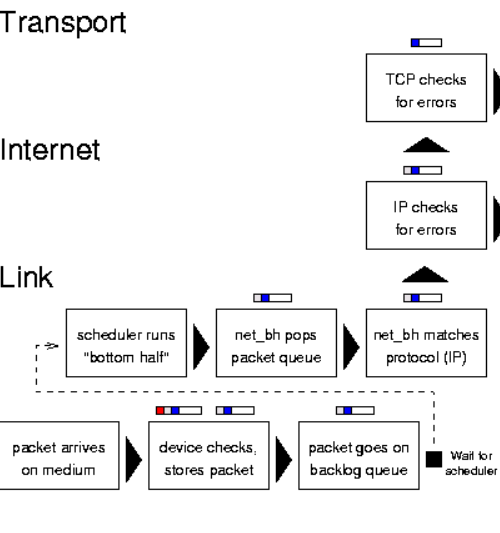
\includegraphics[scale=0.9]{r_rx.png}
	\caption{Обработка входящего пакета}
	\label{rx}
\end{figure}
\indent Исходящий же пакет можно перенаправить на обработку в другой интерфейс с помощью подмены поля dev в структуре sk\_buff.

\subsection{Вывод}
В результате проведенного анализа было определено:
\begin{itemize}
	\item основной структурой сетевой подсистемы Linux является struct net\_device;
	\item функции для работы со struct net\_device определены в \\ struct net\_device\_ops, на которую есть ссылка в struct net\_device;
	\item была выбрана функция инициализации void ether\_setup(struct net\_device *dev);
	\item для реализации задачи были выбраны три функции работы с сетевыми интерфейсами (ndo\_open, ndo\_close, ndo\_start\_xmit).
\end{itemize}
Были проанализированы особенности работы сетевой подсистемы Linux. Проанализирована структура struct net\_device, позволяющая создавать виртуальное сетевое устройство. Была проанализирована структура struct net\_device\_ops, хранящая функции работы с struct net\_device.

\clearpage
\section{Конструкторский раздел}
\subsection{IDEF0}
В системе можно выделить два основных модуля. Модуль получения и модуль отправки пакета. Далее приведены схемы IDEF0 выделенных модулей.
\begin{figure}[H]
	\centering
	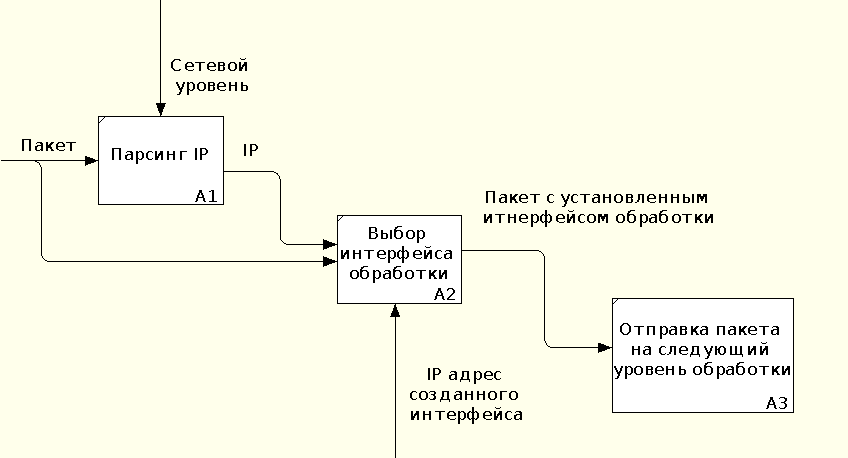
\includegraphics[scale=0.7]{idefin.png}
	\caption{IDEF0 получения пакета}
	\label{idefin}
\end{figure}
\begin{figure}[H]
	\centering
	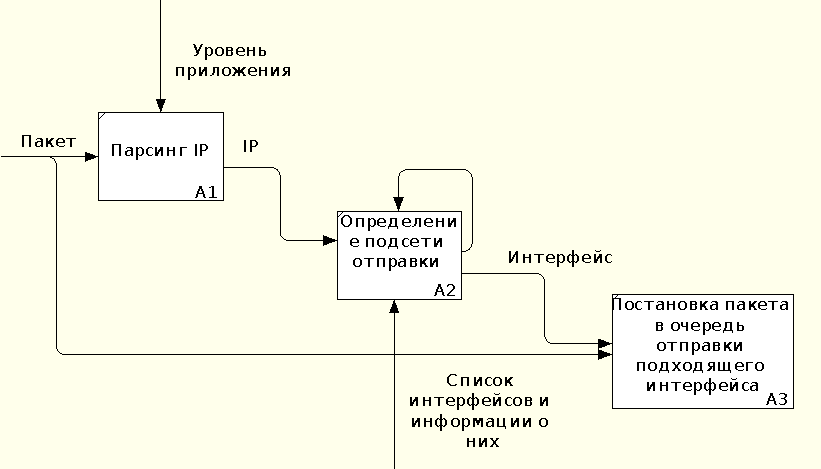
\includegraphics[scale=0.7]{idefout.png}
	\caption{IDEF0 отправки пакета}
	\label{idefout}
\end{figure}

\subsection{Алгоритм получения пакета}
Схема алгоритма обработки принимаемого пакета на одном из интерфейсов, скрываемых виртуальным представлена на рисунке \ref{in}.
\begin{figure}[H]
	\centering
	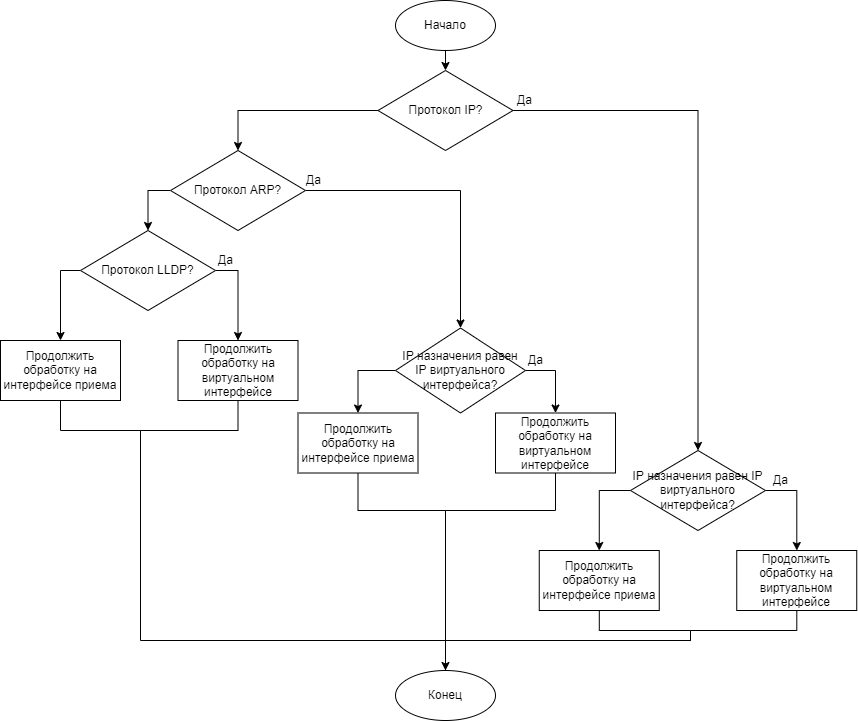
\includegraphics[scale=0.5]{in.png}
	\caption{Схема алгоритма обработки принимаемого пакета}
	\label{in}
\end{figure}

\subsection{Алгоритм отправки пакета}
Так как необходимо хранить информацию о нескольких интерфейсах, было принято решение использовать связанный список, элементами которого будет информация о интерфейсе. \\
\indent Схема алгоритма обработки отправляемого пакета, поступившего на виртуальный интерфейс представлена на рисунке \ref{out}.
\begin{figure}[H]
	\centering
	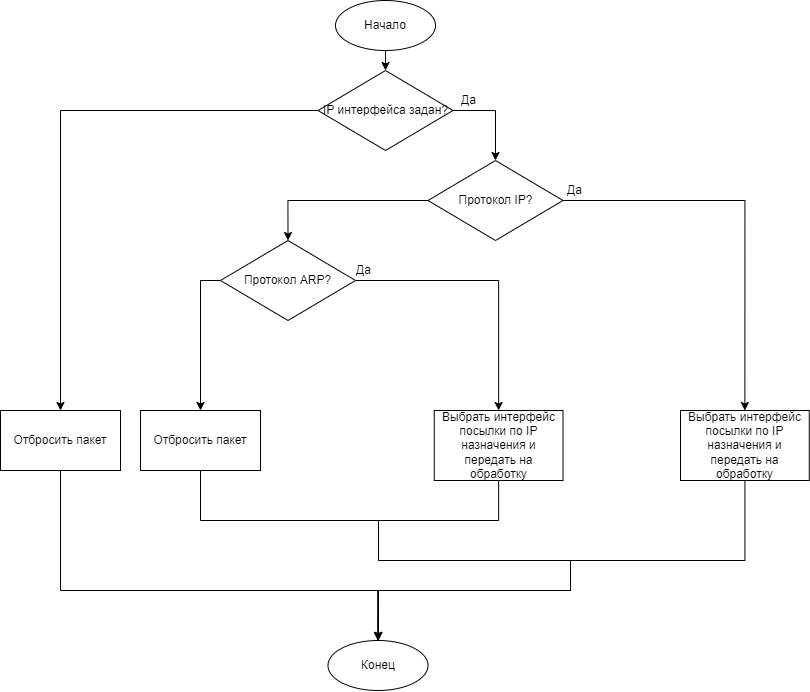
\includegraphics[scale=0.6]{out.png}
	\caption{Схема алгоритма обработки отправляемого пакета}
	\label{out}
\end{figure}

\subsection{Алгоритм инициализации }
\indent Схема алгоритма инициализации структур для работы \ref{gen}.
\begin{figure}[H]
	\centering
	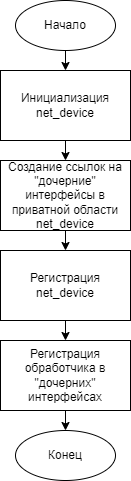
\includegraphics[scale=0.9]{gen.png}
	\caption{Схема алгоритма инициализации структур для работы}
	\label{gen}
\end{figure}

\clearpage
\section{Технологический раздел}
\subsection{Выбор языка программирования и среды программирования}
В качестве языка программирования для реализации поставленной
задачи был выбран язык С. Он является языком реализации модулей ядра и самого ядра ОС Linux. В качестве компилятора был использован
компилятор gcc. Средой разработки был выбран текстовый редактор Visual Studio Code.

\subsection{Описание основных структур}
Для реализации хранения нескольких интерфейсов для распределения пакетов было принято решение хранить в связанном списке ссылки на структуры net\_device и дополнительную информацию об этих интерфейсах. Голова связанного списка хранится в приватной зоне памяти создаваемого виртуального интерфейса. На листинге \ref{linkd} Приведена структура узла вышеупомянутого связанного списка.

\begin{lstlisting}[caption=struct interfaces, label={linkd}]
	struct interfaces {
		u32 address; // адрес подсети
		u32 mask;    // маска подсети
		struct net_device *device; // ссылка на интерфейс
		struct interfaces *next;   // следующий узел
	};
\end{lstlisting}

В приватной области памяти создаваемого виртуального сетевого интерфейса создается структура priv, хранящая статистику интерфейса и начало связанного списка интерфейсов для распределения пакетов. На листинге \ref{priv} представлена структура priv.
\begin{lstlisting}[caption=Структура приватной области интерфейса, label=priv]
	struct priv
	{
		struct net_device_stats stats;
		struct interfaces *next;
	};
\end{lstlisting}

\subsection{Реализация алгоритма получения пакета}
В соответствии с алгоритмом из конструкторской части была спроектирована функция получения пакета. \\
\indent Для избежания блокировки используемых интерфейсов необходимо передавать в созданный интерфейс только пакеты, предназначенные ему. Для этого в функции получения пакета производится проверка на соответствие IP. На листинге \ref{catch} представлена функция получения пакета.
\begin{lstlisting}[caption=Функция получения, label=catch]
	tatic rx_handler_result_t handle_frame(struct sk_buff **pskb)
	{
		struct sk_buff *skb = *pskb;
		struct in_device *in_dev = child->ip_ptr;
		struct in_ifaddr *ifa = in_dev->ifa_list;
		if (!ifa)
		{
			return RX_HANDLER_PASS;
		}
		u32 child_ip = ifa->ifa_address;
		if (skb->protocol == htons(ETH_P_IP))
		{
			struct iphdr *ip = ip_hdr(skb);
			LOG("INCOME: IP to IP=%s", strIP(ip->daddr));
			if (!ifa || ip->daddr != child_ip)
			{
				return RX_HANDLER_PASS;
			}
		}
		else if (skb->protocol == htons(ETH_P_ARP))
		{
			struct arphdr *arp = arp_hdr(skb);
			struct arp_eth_body *body = (void *)arp + sizeof(struct arphdr);
			int i, ip = child_ip;
			LOG("INCOME: ARP for IP=%s", strAR_IP(body->ar_tip));
			for (i = 0; i < sizeof(body->ar_tip); i++)
			{
				if ((ip & 0xFF) != body->ar_tip[i])
				break;
				ip = ip >> 8;
			}
			if (i < sizeof(body->ar_tip))
			return RX_HANDLER_PASS;
		}
		else if (skb->protocol != htons(0xCC88))
		{
			return RX_HANDLER_PASS;
		}
		
		LOG("INCOME: PASS");
		struct priv *priv = netdev_priv(child);
		priv->stats.rx_packets++;
		priv->stats.rx_bytes += skb->len;
		skb->dev = child;
		return RX_HANDLER_ANOTHER;
	}
\end{lstlisting}

\subsection{Реализация алгоритма отправки пакета}
В соответствии с алгоритмом из конструкторской части была спроектирована функция отправки пакета. \\
\indent Функция обработки входящего пакета в создаваемый сетевой интерфейс представлена на листинге \ref{in_l}. Видно, что при нахождении подходящего интерфейса меняется поле dev структуры sk\_buff, а затем буфер отправляется на дальнейшую обработку функцией dev\_queue\_xmit.
\begin{lstlisting}[caption=start\_xmit, label=in_l]
	static netdev_tx_t start_xmit(struct sk_buff *skb, struct net_device *dev)
	{
		struct in_device *in_dev = child->ip_ptr;
		struct in_ifaddr *ifa = in_dev->ifa_list;
		if (ifa) 
		{
			struct priv *priv = netdev_priv(dev);
			priv->stats.tx_packets++;
			priv->stats.tx_bytes += skb->len;
			LOG("GET IP %d, %s", get_ip(skb), strIP(get_ip(skb)));
			struct net_device *device = find_device_sub(priv->next, get_ip(skb));
			if (device)
			{
				skb->dev = device;
				skb->priority = 1;
				dev_queue_xmit(skb);
				LOG("OUTPUT: injecting frame from %s to %s. Tarhet IP: %s", dev->name, skb->dev->name, strIP(get_ip(skb)));
				return NETDEV_TX_OK;
			}
		}
		return NETDEV_TX_OK;
	}
\end{lstlisting}

\subsection{Реализация алгоритма инициализации}
В соответствии с алгоритмом из конструкторской части была спроектирована функция инициализации необходимых структур.\\
\indent Функция init, вызываемая при загрузке модуля и производящая первичную инициализацию, представлена на листинге \ref{init_m}. В функции загрузки модуля происходит вызов функций инициализации и добавление элементов в связный список интерфейсов. Также происходит регистрация виртуального интерфейса и установка функции обработчика пакетов в связанные интерфейсы. 
\begin{lstlisting}[caption=Функции загрузки и выгрузки модуля; label=init_m]
	int __init init(void)
	{
		int err = 0;
		struct priv *priv;
		char ifstr[40];
		sprintf(ifstr, "%s%s", ifname, "%d");
		
		child = alloc_netdev(sizeof(struct priv), ifstr, NET_NAME_UNKNOWN, setup);
		if (child == NULL)
		{
			ERR("%s: allocate error", THIS_MODULE->name);
			return -ENOMEM;
		}
		priv = netdev_priv(child);
		struct net_device *device = __dev_get_by_name(&init_net, link); // parent interface
		if (!device)
		{
			ERR("%s: no such net: %s", THIS_MODULE->name, link);
			err = -ENODEV;
			free_netdev(child);
			return err;
		} else if (device->type != ARPHRD_ETHER && device->type != ARPHRD_LOOPBACK)
		{
			ERR("%s: illegal net type", THIS_MODULE->name);
			err = -EINVAL;
			free_netdev(child);
			return err;
		}
		
		struct interfaces *second = kmalloc(sizeof(struct interfaces), GFP_KERNEL);
		second->address = charToIP(0, 0, (char)0, (char)0);
		second->mask = charToIP(0, 0, (char)0, (char)0);
		second->device = device;
		second->next = NULL;
		
		struct interfaces *first = kmalloc(sizeof(struct interfaces), GFP_KERNEL);
		first->address = charToIP(192, 168, (char)1, (char)0);
		first->mask = charToIP(255, 255, (char)255, (char)0);
		first->device = device;
		first->next = second;
		
		priv->next = first;
		memcpy(child->dev_addr, device->dev_addr, ETH_ALEN);
		memcpy(child->broadcast, device->broadcast, ETH_ALEN);
		if ((err = dev_alloc_name(child, child->name)))
		{
			ERR("%s: allocate name, error %i", THIS_MODULE->name, err);
			err = -EIO;
			free_netdev(child);
			return err;
		}
		register_netdev(child);
		rtnl_lock();
		netdev_rx_handler_register(device, &handle_frame, NULL);
		rtnl_unlock();
		LOG("module %s loaded", THIS_MODULE->name);
		LOG("%s: create link %s", THIS_MODULE->name, child->name);
		LOG("%s: registered rx handler for %s", THIS_MODULE->name, priv->next->device->name);
		return 0;
	}
\end{lstlisting}

\subsection{Дополнительные функции}
Для поиска подходящего интерфейса по связанному списку была написана функция find\_device\_sub. В ней осуществляется проверка принадлежности адреса назначения к подсети по этому интерфейсу. Она представлена на листинге \ref{fds}.

\begin{lstlisting}[caption=find\_device\_sub, label=fds]
static struct net_device *find_device_sub(struct interfaces *subs, u32 addr)
{
    struct net_device *device = NULL;
    while (subs && !device)
    {
        u32 res = apply_mask(subs->mask, addr);
        if (res == subs->address)
        {
            device = subs->device;
        }
        else
        {
            subs = subs->next;
        }
    }

    return device;
}
\end{lstlisting}

На листинге \ref{init} показана инициализация структуры net\_device\_ops и определение оставшихся необходимых функций.

\begin{lstlisting}[caption=net\_device\_ops, label=init]
static int open( struct net_device *dev ) {
   netif_start_queue( dev );
   LOG( "%s: device opened", dev->name );
   return 0;
}

static int stop(struct net_device *dev)
{
    netif_stop_queue(dev);
    LOG("%s: device closed", dev->name);
    return 0;
}

static struct net_device_stats *get_stats(struct net_device *dev)
{
    return &((struct priv *)netdev_priv(dev))->stats;
}

static struct net_device_ops crypto_net_device_ops = {
    .ndo_open = open,
    .ndo_stop = stop,
    .ndo_get_stats = get_stats,
    .ndo_start_xmit = start_xmit,
};
\end{lstlisting}

Полный текст программы можно посмотреть в Приложении А.
\subsection{Makefile}
В листинге \ref{makef} приведен файл Makefile, используемый для сборки модуля ядра.
\begin{lstlisting}[caption=Makefile, label=makef]
CURRENT = $(shell uname -r)
KDIR = /lib/modules/$(CURRENT)/build
PWD = $(shell pwd)
MAKE = make

TARGET1 = cvirt
obj-m := $(TARGET1).o

all: default clean

default:
	$(MAKE) -C $(KDIR) M=$(PWD) modules 

clean:
	@rm -f *.o .*.cmd .*.flags *.mod.c *.order
	@rm -f .*.*.cmd *.symvers *~ *.*~ TODO.*
	@rm -fR .tmp*
	@rm -rf .tmp_versions

disclean: clean
	@rm -f *.ko
\end{lstlisting}

\section{Исследовательская часть}
На рисунке \ref{load} показана загрузка модуля в ядро.

\begin{figure}[H]
	\centering
	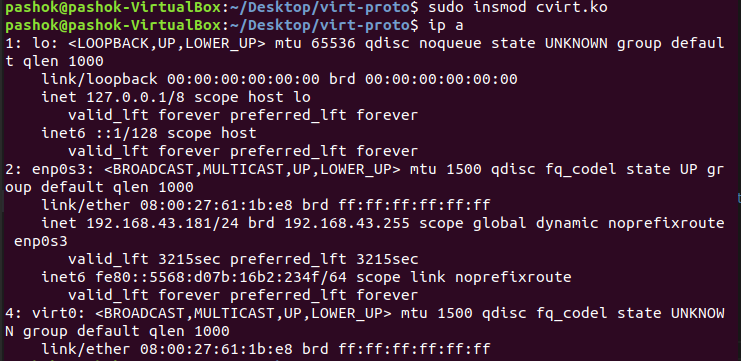
\includegraphics[scale=0.8]{load.png}
	\caption{Загрузка модуля в ядро}
	\label{load}
\end{figure}

На рисунке \ref{sett} и \ref{sett_route} показана настройка интерфейса для приема и передачи пакетов.

\begin{figure}[H]
	\centering
	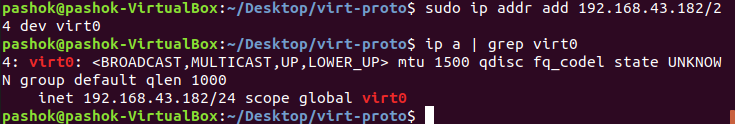
\includegraphics[scale=0.8]{sett.png}
	\caption{Присвоение адреса интерфейсу}
	\label{sett}
\end{figure}

\begin{figure}[H]
	\centering
	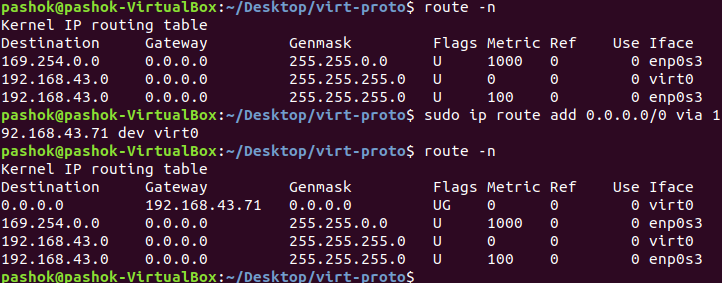
\includegraphics[scale=0.8]{sett_route.png}
	\caption{Добавление пути в таблицу путей Linux}
	\label{sett_route}
\end{figure}

На рисунке \ref{ping} показано, что через виртуальный интерфейс теперь можно получить доступ к машинам с внешним IP. А на рисунке \ref{dmesg} показаны логи ядра, показывающие, что действительно происходит распределение по интерфейсам.
\begin{figure}[H]
	\centering
	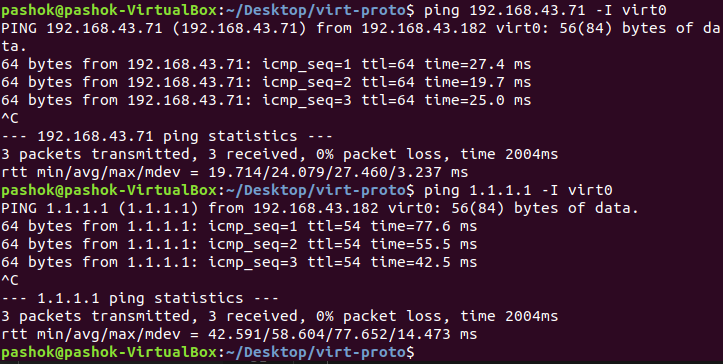
\includegraphics[scale=0.8]{ping.png}
	\caption{Ping}
	\label{ping}
\end{figure}

\begin{figure}[H]
	\centering
	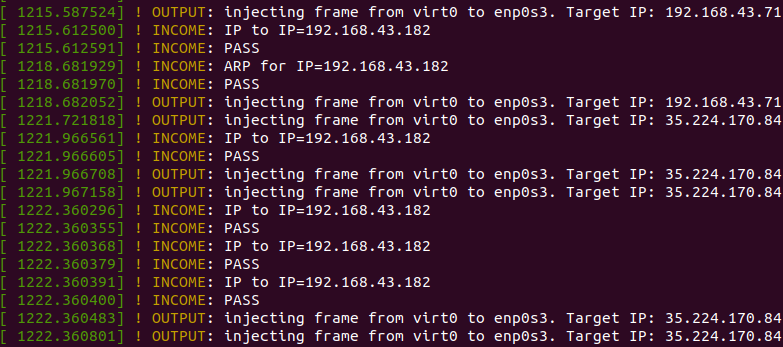
\includegraphics[scale=0.7]{dmesg.png}
	\caption{Логи ядра}
	\label{dmesg}
\end{figure}

\clearpage
\section*{Заключение}
\addcontentsline{toc}{section}{Заключение}
В процессе выполнения курсовой работы по курсу операционные системы был реализован загружаемый модуль ядра для распределения пакетов по существующим интерфейсам. \\
\indent Проанализирована сетевая подсистема Linux, изучены структуры, позволяющие работать с виртуальными сетевыми интерфейсам. \\
\indent Сетевой интерфейс был разработан и реализован, была показана его работоспособность.
\clearpage
\begin{thebibliography}{9}
	\addcontentsline{toc}{section}{Литература}
	\bibitem{ring} Andrew S. Tanenbaum,
Herbert BOS //  Modern Operating Systems FOURTH EDITION c. 479-480.
	\bibitem{ldd-trans} Типы устройств ОС Linux [Электронный ресурс] URL: http://dmilvdv.narod.ru/Translate/LDD3/ldd\_classes\_devices\_modules.html (дата обращения: 22.12.2021).
	
	\bibitem{ldd-orig} Jonathan Corbet, Alessandro Rubini, Greg Kroah-Hartman // Linux Drivers Development, Third Edition c.497.
	
	\bibitem{ldd-setup} Jonathan Corbet, Alessandro Rubini, Greg Kroah-Hartman // Linux Drivers Development, Third Edition c.503.
	
	\bibitem{tuntap} TUN/TAP интерфейсы [Электронный ресурс] URL: https://www.kernel.org/doc/html/latest/networking/tuntap.html (дата обращения: 22.12.2021).
	\bibitem{netdevice} netdevice.h. Исходный код ядра v5.4 [Электронный ресурс] URL: https://elixir.bootlin.com/linux/v5.4/source/include/linux/netdevice.h (дата обращения: 22.12.2021). 22.12.2021).
\end{thebibliography}

\clearpage
\section*{Приложение А}
\addcontentsline{toc}{section}{Приложение А}
\begin{lstlisting}[caption=Полный код разработанного модуля ядра]
	#include <linux/module.h>
	#include <linux/moduleparam.h>
	#include <linux/inetdevice.h> //if_addr
	#include <net/ip.h>
	
	static char *link = "enp0s3"; // имя родительского интерфейса
	module_param(link, charp, 0);
	
	static char *ifname = "virt"; // имя создаваемого интерфейса
	module_param(ifname, charp, 0);
	
	static struct net_device *child = NULL;
	struct interfaces {
		u32 address; // адрес подсети
		u32 mask;    // маска подсети
		struct net_device *device; // ссылка на интерфейс
		struct interfaces *next;   // следующий узел
	};
	
	struct priv
	{
		struct net_device_stats stats;
		struct interfaces *next;
	};
	
	struct arp_eth_body {
		unsigned char  ar_sha[ ETH_ALEN ];     // sender hardware address      
		unsigned char  ar_sip[ 4 ];            // sender IP address            
		unsigned char  ar_tha[ ETH_ALEN ];     // target hardware address      
		unsigned char  ar_tip[ 4 ];            // target IP address            
	};
	
	#define ERR(...) printk(KERN_ERR "! "__VA_ARGS__)
	#define LOG(...) printk(KERN_INFO "! "__VA_ARGS__)
	
	static u32 apply_mask(u32 addr, u32 mask)
	{
		return (addr & mask);
	}
	static char *strIP(u32 addr);
	static struct net_device *find_device_sub(struct interfaces *subs, u32 addr)
	{
		struct net_device *device = NULL;
		while (subs && !device)
		{
			u32 res = apply_mask(subs->mask, addr);
			if (res == subs->address)
			{
				device = subs->device;
			}
			else
			{
				subs = subs->next;
			}
		}
		
		return device;
	}
	
	
	
	static char *strIP(u32 addr)
	{ // диагностика IP в точечной нотации
		static char saddr[MAX_ADDR_LEN];
		sprintf(saddr, "%d.%d.%d.%d",
		(addr)&0xFF, (addr >> 8) & 0xFF,
		(addr >> 16) & 0xFF, (addr >> 24) & 0xFF);
		return saddr;
	}
	
	static char* strAR_IP( unsigned char addr[ 4 ] ) {
		static char saddr[ MAX_ADDR_LEN ];
		sprintf( saddr, "%d.%0d.%d.%d",
		addr[ 0 ], addr[ 1 ], addr[ 2 ], addr[ 3 ] );
		return saddr;
	}
	
	static void print_ip(struct sk_buff *skb)
	{
		if (skb->protocol == htons(ETH_P_IP))
		{
			struct iphdr *ip = ip_hdr(skb);
			char daddr[MAX_ADDR_LEN], saddr[MAX_ADDR_LEN];
			strcpy(daddr, strIP(ip->daddr));
			strcpy(saddr, strIP(ip->saddr));
			LOG("re: from IP=%s to IP=%s with length: %u", saddr, daddr, skb->len);
		}
		else if (skb->protocol == htons(ETH_P_ARP))
		{
			struct arphdr *arp = arp_hdr(skb);
			struct arp_eth_body *body = (void *)arp + sizeof(struct arphdr);
			LOG("re: ARP for %s", strAR_IP(body->ar_tip));
		}
		return 0;
	}
	
	static u32 charToIP( unsigned char fir, unsigned char sec, unsigned char thd, unsigned char frth ) {
		u32 fourth = frth;
		u32 third = thd;
		u32 second = sec;
		u32 first = fir;
		LOG("%d %d", (fourth << 24) | (third << 16), (second << 8) | first);
		return  (fourth << 24)  | (third << 16) | (second << 8) | (first);
	}
	
	static u32 get_ip(struct sk_buff *skb)
	{
		if (skb->protocol == htons(ETH_P_IP))
		{
			struct iphdr *ip = ip_hdr(skb);
			return (ip->daddr);//&0xFF | (ip->daddr >> 8) & 0xFF |
			//(ip->daddr >> 16) & 0xFF | (ip->daddr >> 24) & 0xFF;
		}
		else if (skb->protocol == htons(ETH_P_ARP))
		{
			struct arphdr *arp = arp_hdr(skb);
			struct arp_eth_body *body = (void *)arp + sizeof(struct arphdr);
			
			return (body->ar_tip[0]) | (body->ar_tip[1] << 8) | (body->ar_tip[2] << 16) | (body->ar_tip[3] << 24);
		}
	}
	
	static rx_handler_result_t handle_frame(struct sk_buff **pskb)
	{
		struct sk_buff *skb = *pskb;
		struct in_device *in_dev = child->ip_ptr;
		struct in_ifaddr *ifa = in_dev->ifa_list;
		if (!ifa)
		{
			return RX_HANDLER_PASS;
		}
		u32 child_ip = ifa->ifa_address;
		if (skb->protocol == htons(ETH_P_IP))
		{
			struct iphdr *ip = ip_hdr(skb);
			LOG("INCOME: IP to IP=%s", strIP(ip->daddr));
			if (!ifa || ip->daddr != child_ip)
			{
				return RX_HANDLER_PASS;
			}
		}
		else if (skb->protocol == htons(ETH_P_ARP))
		{
			struct arphdr *arp = arp_hdr(skb);
			struct arp_eth_body *body = (void *)arp + sizeof(struct arphdr);
			int i, ip = child_ip;
			LOG("INCOME: ARP for IP=%s", strAR_IP(body->ar_tip));
			for (i = 0; i < sizeof(body->ar_tip); i++)
			{
				if ((ip & 0xFF) != body->ar_tip[i])
				break;
				ip = ip >> 8;
			}
			if (i < sizeof(body->ar_tip))
			return RX_HANDLER_PASS;
		}
		else if (skb->protocol != htons(0xCC88))
		{
			return RX_HANDLER_PASS;
		}
		
		LOG("INCOME: PASS");
		struct priv *priv = netdev_priv(child);
		priv->stats.rx_packets++;
		priv->stats.rx_bytes += skb->len;
		skb->dev = child;
		return RX_HANDLER_ANOTHER;
	}
	
	static int open( struct net_device *dev ) {
		netif_start_queue( dev );
		LOG( "%s: device opened", dev->name );
		return 0;
	}
	
	static int stop(struct net_device *dev)
	{
		netif_stop_queue(dev);
		LOG("%s: device closed", dev->name);
		return 0;
	}
	
	static netdev_tx_t start_xmit(struct sk_buff *skb, struct net_device *dev)
	{
		struct in_device *in_dev = child->ip_ptr;
		struct in_ifaddr *ifa = in_dev->ifa_list;
		if (ifa) 
		{
			struct priv *priv = netdev_priv(dev);
			priv->stats.tx_packets++;
			priv->stats.tx_bytes += skb->len;
			struct net_device *device = find_device_sub(priv->next, get_ip(skb));
			if (device)
			{
				skb->dev = device;
				skb->priority = 1;
				dev_queue_xmit(skb);
				LOG("OUTPUT: injecting frame from %s to %s. Target IP: %s", dev->name, skb->dev->name, strIP(get_ip(skb)));
				return NETDEV_TX_OK;
			}
		}
		return NETDEV_TX_OK;
	}
	
	static struct net_device_stats *get_stats(struct net_device *dev)
	{
		return &((struct priv *)netdev_priv(dev))->stats;
	}
	
	static struct net_device_ops crypto_net_device_ops = {
		.ndo_open = open,
		.ndo_stop = stop,
		.ndo_get_stats = get_stats,
		.ndo_start_xmit = start_xmit,
	};
	
	static void setup(struct net_device *dev)
	{
		int j;
		ether_setup(dev);
		memset(netdev_priv(dev), 0, sizeof(struct priv));
		dev->netdev_ops = &crypto_net_device_ops;
		for (j = 0; j < ETH_ALEN; ++j) // Заполнить MAC адрес
		{
			dev->dev_addr[j] = (char)j;
		}
	}
	
	int __init init(void)
	{
		int err = 0;
		struct priv *priv;
		char ifstr[40];
		sprintf(ifstr, "%s%s", ifname, "%d");
		
		child = alloc_netdev(sizeof(struct priv), ifstr, NET_NAME_UNKNOWN, setup);
		if (child == NULL)
		{
			ERR("%s: allocate error", THIS_MODULE->name);
			return -ENOMEM;
		}
		priv = netdev_priv(child);
		struct net_device *device = __dev_get_by_name(&init_net, link); // parent interface
		if (!device)
		{
			ERR("%s: no such net: %s", THIS_MODULE->name, link);
			err = -ENODEV;
			free_netdev(child);
			return err;
		} else if (device->type != ARPHRD_ETHER && device->type != ARPHRD_LOOPBACK)
		{
			ERR("%s: illegal net type", THIS_MODULE->name);
			err = -EINVAL;
			free_netdev(child);
			return err;
		}
		
		struct interfaces *second = kmalloc(sizeof(struct interfaces), GFP_KERNEL);
		second->address = charToIP(0, 0, (char)0, (char)0);
		second->mask = charToIP(0, 0, (char)0, (char)0);
		second->device = device;
		second->next = NULL;
		
		struct interfaces *first = kmalloc(sizeof(struct interfaces), GFP_KERNEL);
		first->address = charToIP(192, 168, (char)43, (char)71);
		first->mask = charToIP(255, 255, (char)255, (char)0);
		first->device = device;
		first->next = second;
		
		priv->next = first;
		memcpy(child->dev_addr, device->dev_addr, ETH_ALEN);
		memcpy(child->broadcast, device->broadcast, ETH_ALEN);
		if ((err = dev_alloc_name(child, child->name)))
		{
			ERR("%s: allocate name, error %i", THIS_MODULE->name, err);
			err = -EIO;
			free_netdev(child);
			return err;
		}
		register_netdev(child);
		rtnl_lock();
		netdev_rx_handler_register(device, &handle_frame, NULL);
		rtnl_unlock();
		LOG("module %s loaded", THIS_MODULE->name);
		LOG("%s: create link %s", THIS_MODULE->name, child->name);
		LOG("%s: registered rx handler for %s", THIS_MODULE->name, priv->next->device->name);
		return 0;
	}
	
	void __exit exit(void)
	{
		struct priv *priv = netdev_priv(child);
		struct interfaces *next = priv->next;
		while (next)
		{
			rtnl_lock();
			netdev_rx_handler_unregister(next->device);
			rtnl_unlock();
			LOG("unregister rx handler for %s\n", next->device->name);
			next = next->next;
		}
		unregister_netdev(child);
		free_netdev(child);
		LOG("module %s unloaded", THIS_MODULE->name);
	}
	
	module_init(init);
	module_exit(exit);
	
	MODULE_AUTHOR("Pavel Khetagurov");
	MODULE_LICENSE("GPL v2");
	MODULE_VERSION("0.1");
\end{lstlisting}


\end{document}




